\documentclass[runningheads]{llncs}
\usepackage[T1]{fontenc}
\usepackage{amsmath,amssymb}
\usepackage{booktabs}
\usepackage{graphicx}
\usepackage{xcolor}
\usepackage[colorlinks=true,linkcolor=blue!50!black,citecolor=blue!50!black,urlcolor=blue!50!black]{hyperref}
\renewcommand\UrlFont{\color{blue!50!black}\rmfamily}
\newcommand{\nDev}{328}
\newcommand{\nTest}{768}
\newcommand{\nTasks}{1096}
\newcommand{\tunedSim}{0.8}
\newcommand{\tunedTrust}{0.0}
\newcommand{\tunedEv}{0.1}
\newcommand{\tunedStale}{0.05}
\newcommand{\tunedHL}{365}
\newcommand{\devMRR}{0.693}
\newcommand{\devHit}{0.823}
\newcommand{\gridSize}{420}
\newcommand{\hitFiveSnap}{0.641}
\newcommand{\hitOneSnap}{0.378}
\newcommand{\mrrSnap}{0.497}
\newcommand{\hitFiveEmv}{0.684}
\newcommand{\hitOneEmv}{0.406}
\newcommand{\mrrEmv}{0.532}
\newcommand{\hitFiveTuned}{0.751}
\newcommand{\hitOneTuned}{0.454}
\newcommand{\mrrTuned}{0.585}
\newcommand{\hitFivePlain}{0.551}
\newcommand{\hitOnePlain}{0.333}
\newcommand{\mrrPlain}{0.433}
\newcommand{\hitFiveNaive}{0.612}
\newcommand{\hitOneNaive}{0.357}
\newcommand{\mrrNaive}{0.470}
\newcommand{\hitFivePop}{0.451}
\newcommand{\hitOnePop}{0.083}
\newcommand{\mrrPop}{0.244}
\newcommand{\hitFiveRec}{0.451}
\newcommand{\hitOneRec}{0.189}
\newcommand{\mrrRec}{0.307}
\newcommand{\deadPlain}{0.179}
\newcommand{\deadNaive}{0.181}
\newcommand{\deadBlind}{0.015}
\newcommand{\contamPlain}{0.267}
\newcommand{\deadShare}{20}
\newcommand{\plainDeadTasks}{54}
\newcommand{\shufSnapFive}{0.130}
\newcommand{\shufEmvFive}{0.461}
\newcommand{\leakSnapOne}{0.999}
\newcommand{\leakEmvOne}{0.999}
\newcommand{\trustMean}{1.000}
\newcommand{\trustECE}{0.594}
\newcommand{\aurocGapEmv}{0.751}
\newcommand{\aurocGapSnap}{0.820}
\newcommand{\aurocGapTuned}{0.783}
\newcommand{\aurocTrustEmv}{0.500}
\newcommand{\covTwentyEmv}{0.3}
\newcommand{\accTwentyEmv}{100.0}
\newcommand{\covTwentyTuned}{5.1}
\newcommand{\accTwentyTuned}{97.4}
\newcommand{\covTwentySnap}{6.2}
\newcommand{\accTwentySnap}{93.8}
\newcommand{\covTenEmv}{5.7}
\newcommand{\accTenEmv}{93.2}
\newcommand{\covTenTuned}{14.3}
\newcommand{\accTenTuned}{92.7}
\newcommand{\covTenSnap}{16.7}
\newcommand{\accTenSnap}{88.3}
\newcommand{\covFiveEmv}{15.9}
\newcommand{\accFiveEmv}{86.1}
\newcommand{\covFiveTuned}{29.6}
\newcommand{\accFiveTuned}{82.8}
\newcommand{\covFiveSnap}{31.5}
\newcommand{\accFiveSnap}{74.8}
\newcommand{\dTunedSnapFive}{0.111}
\newcommand{\dTunedSnapLo}{0.082}
\newcommand{\dTunedSnapHi}{0.142}
\newcommand{\tunedOnly}{117}
\newcommand{\snapOnly}{32}
\newcommand{\dEmvSnapFive}{0.043}
\newcommand{\dEmvSnapLo}{0.000}
\newcommand{\dEmvSnapHi}{0.086}
\newcommand{\pEmvSnap}{0.112}
\newcommand{\dEmvPlainFive}{0.133}
\newcommand{\dEmvPlainLo}{0.090}
\newcommand{\dEmvPlainHi}{0.176}
\newcommand{\dTunedEmvFive}{0.068}
\newcommand{\dTunedEmvLo}{0.038}
\newcommand{\dTunedEmvHi}{0.100}
\newcommand{\dTunedSnapOne}{0.077}
\newcommand{\dSnapPlainFive}{0.090}
\newcommand{\ablNoTrust}{+0.021}
\newcommand{\ablNoStale}{+0.035}
\newcommand{\repFastSnap}{0.541}
\newcommand{\repFastEmv}{0.645}
\newcommand{\repFastTuned}{0.715}
\newcommand{\repFastPop}{0.640}
\newcommand{\repFastPlain}{0.384}
\newcommand{\repYtdlpSnap}{0.801}
\newcommand{\repYtdlpEmv}{0.689}
\newcommand{\repYtdlpTuned}{0.893}
\newcommand{\repYtdlpPop}{0.260}
\newcommand{\repYtdlpPlain}{0.796}
\newcommand{\repBuSnap}{0.605}
\newcommand{\repBuEmv}{0.698}
\newcommand{\repBuTuned}{0.698}
\newcommand{\repBuPop}{0.463}
\newcommand{\repBuPlain}{0.502}
\newcommand{\nClaims}{1750}

\graphicspath{{figures/}}
\setlength{\emergencystretch}{3em}
\newcommand{\sys}{EmemoVeri}
\hyphenation{Ememo-Veri}
\setlength{\textfloatsep}{8pt plus 2pt minus 2pt}\setlength{\floatsep}{8pt plus 2pt minus 2pt}\setlength{\intextsep}{8pt plus 2pt minus 2pt}
\renewcommand{\topfraction}{0.9}\renewcommand{\bottomfraction}{0.9}\renewcommand{\textfraction}{0.1}\renewcommand{\floatpagefraction}{0.8}
\begin{document}
\title{Retrieving Over Evidence Items: Repository Memory for Coding Agents, Evaluated on Real Git History}
\titlerunning{Retrieving Over Evidence Items}
\author{Mihit \and Priyanka Tyagi}
\authorrunning{M. Mihit and P. Tyagi}
\institute{IILM University, Greater Noida, India\\
\email{mihit.nanda.cs27@iilm.edu}}
\maketitle
\begin{abstract}
A coding agent that works on one repository for a long time needs a memory of it. That memory has to cope with files that are renamed or deleted, changes that are reverted, and old knowledge that is no longer true. We study such a memory, called \sys{}, on a benchmark built from real git history. At each step the memory sees only the past and must rank the files that a \emph{future} commit will change. We first show that the original \sys{} scorer is no better than a simple tuned baseline, and that its trust and abstention parts carry no useful signal. We then redesign it so that retrieval runs on the memory's evidence records themselves: each past commit is compared with the query, and a file inherits the score of its best-matching commit. We fix this design using three repositories, then test it, without any change, on 16 repositories that were never used before (5{,}832 tasks, in Python, JavaScript, Go, Rust and Java). Under a plan written in advance, it ranks the right file in the top five more often than snapshot retrieval (by 0.132 [0.108, 0.155], better in 15 of 16 repositories), the original design (by 0.041 [0.027, 0.057]) and a tuned recency-and-popularity baseline (by 0.043 [0.027, 0.060]), and it is not worse than a gradient-boosted ranker. One refinement that looked helpful during design, weighting evidence by its strength, does not hold up on new data. The result also holds for all 48 weight settings we tried. Code, tests and all results are released.
\end{abstract}
\keywords{Coding agents \and Agent memory \and Repository mining \and Change localisation \and Empirical evaluation}

\section{Introduction}
A coding agent that works on one repository for weeks learns many things: which module owns a behaviour, which function replaced an old one, which test protects a rule. This knowledge goes out of date. Files are renamed or deleted, changes are reverted, and a later commit can overturn what an earlier one showed. A memory that only stores and retrieves text cannot tell an old statement from a current one. \sys{} is a design that tries to fix this. It keeps \emph{evidence} for each remembered fact about a file, and lets the fact's \emph{state} change when new evidence arrives.

Judging such a memory fairly is hard. A realistic test needs a language model in the loop and answers that do not depend on the memory being tested. Synthetic tests are cheap, but if the generator decides the right answer by giving it higher trust, newer timestamps and test evidence, it rewards exactly what the scorer already uses. The first \sys{} experiments had this flaw, so we do not use them. We instead replay the real history of open-source repositories (Section~\ref{sec:bench}) under test plans written before the results exist. The first series showed that the original design does not hold up. The second redesigns retrieval and tests the new design on repositories that had no part in building it.

\textbf{In plain terms.} At a point in a repository's history, the memory is given only the one-line summary (the \emph{subject}) of a commit that has not happened yet. It must guess which source files that commit will change. We call the guess good if a correct file is among the five it ranks first (this is called \emph{Hit@5}). We ask six questions. \textbf{RQ1:} which parts of the original design help, compared with strong simple baselines? \textbf{RQ2:} what happens to the trust and abstention components? \textbf{RQ3:} does retrieving over the evidence records themselves repair the design on repositories never seen before? \textbf{RQ4:} do the extra details stored in the records (strength, type, age, reverts) matter? \textbf{RQ5:} does the result hold for other retrieval methods, other languages, and vague or detailed queries? \textbf{RQ6:} does state tracking handle deleted, renamed and reverted files?

\begin{figure}[t]\centering
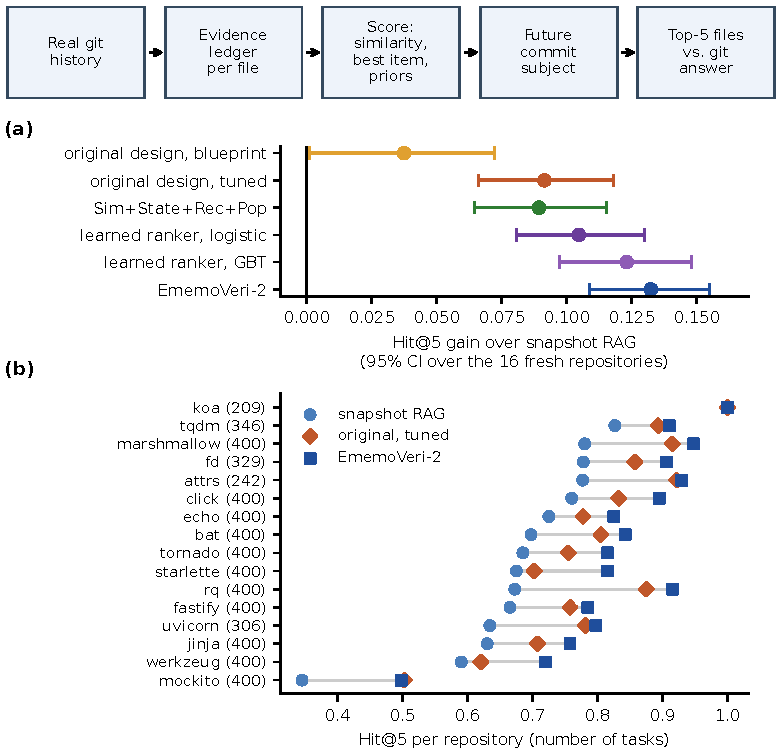
\includegraphics[width=0.84\linewidth]{fig_overview.pdf}
\caption{Overview. Memory is built from git events on one clock and queried with the subject of a future commit. (a) Gain in Hit@5 over snapshot retrieval for systems frozen before testing, on the 16 fresh repositories (95\% intervals from resampling repositories). (b) Hit@5 for each repository, with the number of tasks in brackets.}
\label{fig:overview}
\end{figure}

\noindent Our contributions are:
\begin{enumerate}
\item \textbf{A replay benchmark on real history with built-in checks.} Each task is scored before its own commit is added, and relations and answers come from git. A leak check and a shuffled-query check test the harness. Three test plans written in advance cover 36 repositories in five languages (Section~\ref{sec:bench}).
\item \textbf{A negative result on the original design:} its trust and abstention parts carry no signal, and its scorer is beaten by retrieval over individual evidence records (Sections~\ref{sec:orig} and~\ref{sec:heldout}).
\item \textbf{\sys{}-2, a redesign confirmed on new data}, tested on 16 fresh repositories against five hypotheses stated beforehand. One refinement that helped on development data, evidence-strength weighting, is \emph{not} confirmed (Sections~\ref{sec:ev2} and~\ref{sec:confirm}).
\item \textbf{Robustness and lifecycle checks:} other retrieval methods, vague and detailed queries, deleted and renamed files, and cancelled reverts (Sections~\ref{sec:general} and~\ref{sec:life}).
\item \textbf{An audit} of eight defects in the first implementation, now fixed and tested (Section~\ref{sec:audit}).
\end{enumerate}
We do not claim that \sys{} makes an agent solve more tasks: no language model is in the loop, and queries are commit subjects, not issue reports. The idea of ranking files by the similarity of their past commit subjects to the query comes from bug localisation research~\cite{zhou2012buglocator}. What is new here is running it on a memory that tracks file state and renames, and measuring which stored details actually matter.

\section{Related Work}
\textbf{Memory for language-model agents.} Retrieval-augmented generation~\cite{lewis2020rag} gives a model retrieved passages as context. Agent-memory systems add rules for writing, updating and forgetting. MemGPT moves information between tiers of context~\cite{packer2023memgpt}. Generative Agents rank memories by recency, importance and relevance~\cite{park2023generative}. Reflexion keeps written self-feedback between attempts~\cite{shinn2023reflexion}. Mem0~\cite{chhikara2025mem0} and A-MEM~\cite{xu2025amem} reorganise stored memories as new information arrives. LongMemEval tests long-term recall in chat assistants, including how they handle facts that change~\cite{wu2024longmemeval}. These systems need a language model and we could not run them; our Sim+State+Rec+Pop baseline is a Generative-Agents-style score with ``importance'' replaced by how often a file changes. Our memory describes a code repository, its updates are version-control events, and the right answers can be read from the history.

\textbf{Repository-level code assistance.} SWE-bench~\cite{jimenez2024swebench} and SWE-agent~\cite{yang2024sweagent} check whether an agent resolves real issues, and RepoCoder~\cite{zhang2023repocoder} retrieves repository context repeatedly during completion. All need a model in the loop; we isolate the memory and measure only which files it brings up.

\textbf{Mining software repositories.} Co-change mining recommends files that tend to change together~\cite{zimmermann2005mining}. Files that changed recently or often are more likely to contain faults~\cite{kim2007cache,hassan2009complexity}. Bug localisation ranks files against a bug report, and one of its components uses similar past reports~\cite{zhou2012buglocator}. Our finding that change frequency and similar-history retrieval are hard to beat agrees with this work. Kalliamvakou et al.~\cite{kalliamvakou2014perils} describe the pitfalls of mining GitHub; like PyDriller~\cite{spadini2018pydriller}, we read history directly with \texttt{git}. Selective classification~\cite{geifman2017selective} and expected calibration error~\cite{guo2017calibration} frame our analysis of abstention and trust.

\section{The \sys{} Mechanism}
\label{sec:mech}
\textbf{Claims, evidence and state.} A \emph{claim} describes one source file. An \emph{evidence item} records one event about it, with a type (commit, test, issue, documentation, agent observation, external), a relation (corroborates, refines, contradicts, supersedes), a time and a strength. A claim starts as PROVISIONAL and becomes CORROBORATED, REFINED or CONTESTED as evidence arrives. SUPERSEDED is final (Section~\ref{sec:audit}). Evidence comes from git events, not from the wording of messages: adding a file corroborates, modifying it refines, deleting it or renaming it away supersedes, and a commit with git's ``This reverts commit'' line contradicts the claims of the files it touches. A rename carries evidence and text over to the new path, and a path that reappears after deletion starts a new claim. Evidence counts as TEST evidence when the same commit also edits a test file. Its strength is 1.0, or 0.3 for bulk commits that touch more than three source files.

\textbf{The original scorer (\sys{}-1).} The text of a claim is the file path plus its five most recent commit subjects. For a query at time $\tau$,
\begin{equation}
s = 0.45\,\mathrm{sim} + 0.25\,\mathrm{trust} + 0.20\,\mathrm{evid} + 0.10\,\mathrm{scope} - 0.10\,\mathrm{stale}.
\end{equation}
Here $\mathrm{sim}$ is the cosine similarity between TF-IDF vectors (hashed unigrams and bigrams) of the query and the claim text. Trust is updated by $t\leftarrow\mathrm{clip}(t+0.35\,w_e,0,1)$. The term $\mathrm{evid}=E/(E+5)$ grows with the total evidence strength $E$. The staleness $\mathrm{stale}=1-2^{-\Delta/90}$ grows with the days $\Delta$ since the last update. Superseded claims are excluded. Because $-w\,\mathrm{stale}=w\,2^{-\Delta/H}-w$, the staleness term is really a recency bonus, and $\mathrm{evid}$ is a strength-weighted count of changes. A conflict resolver abstains when the score gap to the runner-up is below 0.20.

\textbf{\sys{}-2.} The five-subject summary used above throws away most of the evidence. \sys{}-2 compares the query with the subject of \emph{each} evidence item and lets a claim take the score of its best-matching item:
\begin{equation}
s_2(c)=w_s\,\mathrm{sim}(c)+w_e\max_{e\in\mathcal{E}_\tau(c)}\sigma_e\cos(q,\mathrm{subj}_e)+\lambda_p\tfrac{n_c}{n_c+5}+\lambda_r 2^{-\Delta_c/H}.
\end{equation}
Here $\mathcal{E}_\tau(c)$ is the set of items of claim $c$ registered before time $\tau$ (items follow a claim across renames), $\sigma_e\in\{1,0.3\}$ is the item's strength, $n_c$ is the number of changes to the file, and cosines use TF-IDF over the commit subjects registered so far. Only live files in the same repository are ranked. Trust and abstention are dropped. The setting tuned on the development repositories is $w_s=w_e=1$, $\lambda_p=\lambda_r=0.05$ and $H=30$ days. Four further options were searched and are off in the tuned system: a TEST-evidence bonus, a discount by commit size, an item-age decay, and cancelling items whose commit was later reverted (Section~\ref{sec:ev2}).

\section{Benchmark and Protocol}
\label{sec:bench}
\textbf{Task.} At time $t$ the system receives the cleaned subject of a \emph{future} commit $C$. It must rank source files, and its memory contains only commits strictly before $C$. The correct answer is the set of source files that $C$ changed, read from git. Commits are replayed in order, using the running maximum of commit timestamps as the clock (real histories contain timestamps that go backwards). A commit is an eligible task if it is not by a bot, is not a revert, changes one to four tracked files that already have claims, and comes after a warm-up covering the first 35\% of the repository's commits that touch source files. We draw up to 400 evenly spaced tasks per repository. Reverts that touch source files are rare (Table~\ref{tab:data}), so contradictions are tested only lightly.

\begin{table}[t]\centering\footnotesize\setlength{\tabcolsep}{3pt}
\resizebox{\linewidth}{!}{\begin{tabular}{lrrrrrr}
\toprule
Repository & Commits & Source-touching & Eligible & Selected & Cold-file excl. & Clock anomalies \\
\midrule
fastapi & 7,712 & 853 & 296 & 296 & 0 & 12 \\
yt-dlp & 22,449 & 5,052 & 1,885 & 400 & 0 & 2,289 \\
browser-use & 7,003 & 4,057 & 1,773 & 400 & 5 & 4,294 \\
\bottomrule
\end{tabular}}
\caption{Development repositories and task selection. Clock anomalies are commits whose recorded timestamp is earlier than the running clock.}
\label{tab:data}
\end{table}

\textbf{Checks on the benchmark itself.} Memory is updated only after a task is scored, and a runtime check rejects any state that contains evidence newer than the task (it passed on every task in every set). A \emph{leak check} scores each task again after its own commit has been added; a sound harness must then show a big jump, and it does (Hit@1 \leakSnapOne{} for snapshot RAG). A \emph{shuffled-query check} gives each task another task's query. Snapshot RAG then falls to Hit@5 \shufSnapFive{}, but the original blueprint keeps \shufEmvFive{}, about what recency or popularity alone achieves, so part of its score does not depend on the query.

\textbf{Repository sets and test plans.} Table~\ref{tab:sets} lists four sets. The \emph{development} set (fastapi, yt-dlp, browser-use) shaped the code and the baselines. We tune weights on its \emph{dev} part (the earliest 30\% of tasks, \nDev{} tasks) and report on its \emph{test} part (\nTest{} tasks). The \emph{held-out Python} and \emph{multi-language} sets were tested under plans written before their results existed (PROTOCOL\_V04 and V05 in the repository), with every system frozen. These tests were about the original design, and the multi-language run also added the baselines described below. Their results led to \sys{}-2, so for \sys{}-2 they count as \emph{post hoc} (looked at before the design was fixed). The \emph{fresh} set was chosen and configured, \sys{}-2 was frozen, and its five hypotheses were stated, all before any fresh result was computed (PROTOCOL\_V06; the frozen setting is committed and hashed). It is the confirmatory test.

\begin{table}[t]\centering\footnotesize\setlength{\tabcolsep}{3pt}
\begin{tabular}{@{}l p{0.55\linewidth} r p{0.16\linewidth}@{}}
\toprule
Set & Repositories & Tasks & Status for \sys{}-2 \\
\midrule
Development & fastapi, yt-dlp, browser-use & 1{,}096 & tuning (328) / test (768) \\
Held-out Python & flask, requests, httpx, rich, black, poetry, pydantic, scrapy, pytest, aiohttp, celery, sphinx & 4{,}636 & post hoc \\
Multi-language & express, axios (JS); gin, cobra (Go); ripgrep, serde (Rust); jackson-databind, commons-lang (Java) & 3{,}035 & post hoc \\
Fresh & starlette, uvicorn, click, jinja, werkzeug, attrs, tornado, marshmallow, tqdm, rq; koa, fastify (JS); echo (Go); fd, bat (Rust); mockito (Java) & 5{,}832 & \textbf{confirmatory} \\
\bottomrule
\end{tabular}
\caption{Repository sets (36 repositories, five languages).}
\label{tab:sets}
\end{table}

\textbf{Systems and baselines.} We compare against these simple systems. Query-independent priors rank files at random, by most recent change, or by most evidence. \emph{Plain RAG} ranks by text similarity across all repositories and keeps deleted files. \emph{Naive memory} ranks by similarity within one repository and keeps deleted files. \emph{Snapshot RAG} ranks by similarity within one repository and drops deleted files, which is what an agent with a working tree gets for free. The original design is run with its blueprint weights (\sys{}-1-D) and with weights tuned on dev over a \gridSize{}-point grid (\sys{}-1-T).

A family of scores $\mathrm{sim}+\lambda_p\mathrm{pop}+\lambda_e\mathrm{evid}+\lambda_t\mathrm{trust}+\lambda_r 2^{-\Delta/H}$, with or without the state filter, gives the step-by-step ladder and the tuned recency and popularity baselines. Each is tuned on dev by the same rule.

We also adapt established ideas to a commit-subject query (no bug reports exist for this task). \emph{Similar-history retrieval}~\cite{zhou2012buglocator} scores a file by how similar the query is to the subjects of past commits that touched it. \emph{Co-change recommendation}~\cite{zimmermann2005mining} takes the top-ranked file as a seed and scores other files by how often they changed with it. A linear \emph{all-channel} scorer combines every signal, and \emph{learned rankers} (logistic regression and a depth-3 gradient-boosted tree model) use all signals, trained on the 328 dev tasks over the 50 best candidates. Every baseline is tuned or trained on the development dev part only.

\textbf{Metrics and statistics.} Hit@$k$ is the share of tasks where a correct file is among the first $k$ distinct files. We also report MRR, NDCG@5, Recall@5, All@5 (every correct file is in the top five) and Dead@5 (the share of top-five slots occupied by deleted paths). On the development set, paired differences use 10{,}000 bootstrap resamples over tasks, over repository-by-month blocks and over groups of tasks that share a correct file, plus an exact McNemar test with Holm correction. On the other sets the unit of analysis is the \emph{repository}: we report the macro-average (the mean over repositories), a bootstrap over repositories, an exact sign-flip permutation test, Cohen's $d_z$ for the per-repository differences, and Holm correction within each family of hypotheses stated in advance. With $n$ repositories the smallest exact $p$ that can be reached is $2^{1-n}$.

\section{Results: the Original Design}
\label{sec:orig}
\subsection{RQ1: what pays off on the development repositories}
\textbf{Unfiltered retrieval has clear hazards.} Plain RAG puts a file from another repository in \contamPlain{} of its top-five slots, and plain RAG and naive memory put a deleted path in about \deadPlain{} of them (\plainDeadTasks{}\% of test tasks have one in the plain-RAG top five). Dropping deleted files alone (snapshot RAG) raises Hit@5 by \dSnapPlainFive{}. This is a flaw of the baselines, not a finding about state tracking: the filter removes dead paths by construction.

\textbf{Step-by-step ladder.} Table~\ref{tab:ladder} adds one ingredient at a time and re-tunes the added weights on dev. The state filter adds $+0.029$ Hit@5. A change-frequency prior adds $+0.087$, the largest step. Strength-weighted evidence adds $+0.016$ [$-0.001$, $0.033$], trust $-0.003$, and the recency (staleness) term $0.000$.

\begin{table}[t]\centering\footnotesize\setlength{\tabcolsep}{4pt}
\resizebox{\linewidth}{!}{\begin{tabular}{lcccccc l}
\toprule
Rung & Hit@1 & Hit@3 & Hit@5 & MRR & NDCG@5 & Dead@5 & $\Delta$Hit@5 [95\% CI] \\
\midrule
R0 similarity (dead files kept) & 0.357 & 0.531 & 0.612 & 0.470 & 0.462 & 0.181 & -- \\
R1 + state filter & 0.378 & 0.564 & 0.641 & 0.497 & 0.488 & 0.000 & 0.029 [0.017, 0.042] \\
R2 + frequency prior & 0.449 & 0.650 & 0.728 & 0.574 & 0.562 & 0.000 & 0.087 [0.052, 0.122] \\
R3 + evidence & 0.462 & 0.656 & 0.743 & 0.587 & 0.575 & 0.000 & 0.016 [$-$0.001, 0.033] \\
R4 + trust & 0.461 & 0.655 & 0.741 & 0.586 & 0.573 & 0.000 & $-$0.003 [$-$0.007, 0.000] \\
R5 + recency & 0.474 & 0.660 & 0.741 & 0.594 & 0.579 & 0.000 & 0.000 [$-$0.009, 0.009] \\
\midrule
\sys{} dev-tuned (reference) & 0.454 & 0.661 & 0.751 & 0.585 & 0.577 & 0.000 & -- \\
\bottomrule
\end{tabular}}
\caption{Step-by-step ladder for the original design on the development test split. Weights of the added terms are tuned on dev at each step.}
\label{tab:ladder}
\end{table}

\textbf{Strong baselines.} Table~\ref{tab:strong} tunes the strongest baselines that use only simple signals. Change frequency matters more than recency (Sim+Popularity 0.720 against Sim+Recency 0.664), the two complement each other (0.743), and the state filter adds 0.011 (0.754). \emph{The tuned original design (0.751) cannot be told apart from tuned Sim+State+Rec+Pop} ($-0.003$; task CI [$-0.020$, $0.014$]; file-cluster CI [$-0.018$, $0.014$]). With blueprint weights it is only $+0.043$ over snapshot RAG (Holm $p=0.112$), and its intervals include zero under block and file-cluster resampling.

\begin{table}[t]\centering\footnotesize\setlength{\tabcolsep}{4pt}
\resizebox{\linewidth}{!}{\begin{tabular}{lcccll}
\toprule
System & Hit@5 & MRR & NDCG@5 & \multicolumn{2}{c}{\sys{}-T minus system, Hit@5 [95\% CI]} \\
 & & & & task bootstrap & file-cluster bootstrap \\
\midrule
Snapshot RAG & 0.641 & 0.497 & 0.488 & 0.111 [0.081, 0.141] & 0.111 [0.048, 0.166] \\
Sim+Rec & 0.664 & 0.520 & 0.509 & 0.087 [0.060, 0.116] & 0.087 [0.028, 0.141] \\
Sim+Pop & 0.720 & 0.552 & 0.546 & 0.031 [0.009, 0.053] & 0.031 [0.003, 0.068] \\
Sim+Rec+Pop & 0.743 & 0.577 & 0.571 & 0.008 [$-$0.009, 0.025] & 0.008 [$-$0.009, 0.026] \\
Sim+State+Rec & 0.686 & 0.538 & 0.527 & 0.065 [0.036, 0.094] & 0.065 [0.009, 0.118] \\
Sim+State+Pop & 0.728 & 0.574 & 0.562 & 0.023 [0.001, 0.046] & 0.023 [$-$0.008, 0.061] \\
Sim+State+Rec+Pop & 0.754 & 0.585 & 0.578 & $-$0.003 [$-$0.020, 0.014] & $-$0.003 [$-$0.018, 0.014] \\
\sys{}-D (blueprint) & 0.684 & 0.532 & 0.520 & 0.068 [0.036, 0.100] & 0.068 [0.008, 0.142] \\
\midrule
\sys{}-T (dev-tuned) & 0.751 & 0.585 & 0.577 & -- & -- \\
\bottomrule
\end{tabular}}
\caption{Tuned baselines on the development test split. Sim: similarity; State: deleted files removed; Rec: recency; Pop: change frequency. Last columns: Hit@5 of the tuned original design minus the row's system.}
\label{tab:strong}
\end{table}

\textbf{Blueprint ablations.} Removing the trust term or the staleness term of the blueprint \emph{improves} Hit@5 (by $+0.021$ and $+0.035$), and the evidence term cannot be told from zero. Staleness has no simple rule (Fig.~\ref{fig:sweeps}b): a 7--90 day half-life helps tuned weights by at most 0.017 but hurts blueprint weights (0.661 at 7 days against 0.719 without staleness), because the typical top similarity is only 0.12 and a prior weight of 0.10 can drown it out.

\subsection{RQ2: trust and abstention}
\label{sec:trust}
For the top-ranked claim, mean trust is \trustMean{} and its AUROC for predicting a correct top answer is \aurocTrustEmv{}, no better than chance. The update reaches 1 after two or three strong events, and nearly all evidence in the benchmark is positive, so trust cannot separate claims (expected calibration error \trustECE{}, which equals one minus accuracy for a value stuck near 1). The score gap is informative (AUROC \aurocGapEmv{} for the blueprint, \aurocGapTuned{} tuned), but a plain similarity gap on snapshot RAG is better (\aurocGapSnap{}). At the prescribed threshold the blueprint answers \covTwentyEmv{}\% of tasks, the tuned system \covTwentyTuned{}\% and snapshot RAG \covTwentySnap{}\%. We found no sign that either component adds value. We did not design a replacement: this data has no negative or independent evidence on which a new trust model could be checked. Both parts are dropped from \sys{}-2.

\subsection{The original design on untouched repositories (RQ1 continued)}
\label{sec:heldout}
The tests planned in advance on the held-out Python and multi-language sets (systems frozen, repositories as the unit) gave the same picture. The tuned original design beat snapshot RAG by 0.090 [0.064, 0.118] Hit@5 on 12 Python repositories (wins/losses 12/0, Holm $p=0.004$) and by 0.087 [0.049, 0.128] on eight repositories in four other languages (8/0, Holm $p=0.062$; with eight repositories the smallest exact $p$ is 0.008). It again could not be told apart from Sim+State+Rec+Pop ($-$0.004 [$-$0.008, 0.001] and $-$0.004 [$-$0.017, 0.008]), and the blueprint weights were not reliably better than snapshot RAG (0.033 [$-$0.006, 0.073] and 0.024 [$-$0.026, 0.065]). We had predicted that \emph{no} adapted baseline would beat the tuned design. This was wrong: similar-history retrieval mixed with claim similarity and priors beat it by $0.062$ Hit@5 on held-out Python ([0.042, 0.082]; worse in 11 of 12 repositories with one tie) and was within noise on the multi-language set ($-$0.012 [$-$0.030, 0.002]). This led to the redesign below, and it is why these two sets count as post hoc for \sys{}-2.

\begin{figure}[t]\centering
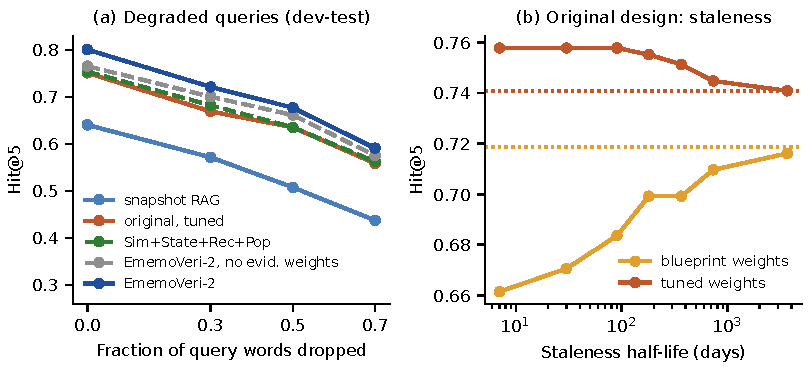
\includegraphics[width=\linewidth]{fig_sweeps2.pdf}
\caption{(a) Hit@5 when each query word is dropped with the given probability (dev-test; weights fixed). (b) Original design: Hit@5 against the staleness half-life; dotted lines show no staleness term.}
\label{fig:sweeps}
\end{figure}

\section{Results: \sys{}-2}
\subsection{RQ3 and RQ4: design on the development split}
\label{sec:ev2}
We designed and tuned \sys{}-2 on the dev split (328 tasks) only, in two stages. First we chose the evidence options (aggregation, strength, discount by commit size, TEST bonus, item decay, revert cancellation) at a fixed blend. Then we tuned the blend (claim similarity, frequency, recency) on a grid. The same grid was also given to a variant with every evidence weight switched off (\sys{}-2 \emph{without evidence weights}), so both had the same tuning budget. On the dev-test split, \sys{}-2 reaches Hit@5 0.801 against 0.766 without evidence weights (0.035 [0.017, 0.053]; file-cluster CI 0.035 [0.014, 0.057]). Inside the tuned system, dropping strength weighting costs 0.029 on that split. A TEST bonus, a commit-size discount and revert cancellation change nothing, and sum or noisy-OR scoring and an item-age decay hurt. On the development set, \sys{}-2 beats snapshot RAG by 0.160 [0.128, 0.194], the original design by 0.049 [0.025, 0.074] and Sim+State+Rec+Pop by 0.047 [0.022, 0.073], and is level with the gradient-boosted ranker (0.004 [$-$0.020, 0.027]). \emph{These numbers are in-sample for the design choices}: the options and the blend were picked on dev, and the baselines come from the same families. This is why the fresh set in Section~\ref{sec:confirm} matters.

\subsection{RQ3 and RQ4: confirmation on 16 fresh repositories}
\label{sec:confirm}
Table~\ref{tab:systems} shows all systems on the fresh set. Table~\ref{tab:contrasts} shows the five hypotheses stated in advance, with Holm correction over H1--H5 (six contrasts).

\textbf{H1 is confirmed.} \sys{}-2 beats snapshot RAG by 0.132 [0.108, 0.155] Hit@5 (better in 15 of 16 repositories; $p<0.001$, Holm $p<0.001$, $d_z=2.68$). The gain is 0.147 [0.126, 0.173] on the 10 Python repositories and 0.108 [0.061, 0.140] on the six in other languages (exact $p=0.062$ with six repositories, where the smallest possible value is 0.031). \textbf{H2 is confirmed:} the redesign beats the original tuned design by 0.041 [0.027, 0.057] (Holm $p<0.001$). \textbf{H4 is confirmed:} it beats Sim+State+Rec+Pop by 0.043 [0.027, 0.060] (Holm $p<0.001$). \textbf{H5:} \sys{}-2 is not worse than the all-channel linear scorer (0.004 [0.000, 0.009]) or the gradient-boosted ranker (0.009 [$-$0.001, 0.020]); both intervals include or touch zero.

\textbf{H3 is not confirmed.} \sys{}-2 beats \sys{}-2 without evidence weights by only 0.001 [$-$0.005, 0.007] (9 wins and 5 losses; $p=0.725$, $d_z=0.09$). The $+0.035$ seen on the dev-test split does not carry over: on new data, evidence strength adds nothing measurable to similar-history retrieval. What works is \emph{retrieving over the evidence items themselves}, together with the state filter, rename carry-over and two cheap priors. The strength attribute is not a measured contributor. The same holds when ``routine'' tasks are removed (377 tasks with duplicate subjects or release and version-bump housekeeping; 5{,}455 tasks remain: H1 0.134 [0.110, 0.158], H3 0.002 [$-$0.005, 0.008], H4 0.043 [0.027, 0.060]).

\begin{table}[t]\centering\footnotesize\setlength{\tabcolsep}{4pt}
\resizebox{\linewidth}{!}{\begin{tabular}{l@{\hspace{4pt}}ccccc|ccc}
\toprule
 & \multicolumn{5}{c|}{Fresh 16 (macro-average)} & \multicolumn{3}{c}{Hit@5 on earlier sets} \\
System (frozen) & Hit@1 & Hit@5 & MRR & NDCG & All@5 & Dev-test & Held-out & Multi. \\
\midrule
Snapshot RAG & 0.381 & 0.703 & 0.523 & 0.516 & 0.590 & 0.641 & 0.603 & 0.640 \\
\midrule
\sys{}-1, blueprint & 0.427 & 0.740 & 0.566 & 0.554 & 0.616 & 0.684 & 0.636 & 0.664 \\
\sys{}-1, tuned & 0.450 & 0.794 & 0.600 & 0.601 & 0.680 & 0.751 & 0.693 & 0.728 \\
\midrule
Sim+State+Rec+Pop & 0.461 & 0.792 & 0.605 & 0.603 & 0.679 & 0.754 & 0.696 & 0.732 \\
Similar-history+priors & 0.504 & 0.828 & 0.644 & 0.645 & 0.716 & 0.772 & 0.755 & 0.740 \\
All channels, linear & 0.512 & 0.831 & 0.649 & 0.650 & 0.721 & 0.772 & 0.761 & 0.747 \\
Ranker, logistic & 0.501 & 0.807 & 0.636 & 0.631 & 0.694 & 0.788 & 0.726 & 0.742 \\
Ranker, GBT & 0.523 & 0.826 & 0.658 & 0.653 & 0.713 & 0.797 & 0.755 & 0.746 \\
\midrule
\sys{}-2, no evid.\ weights & 0.513 & 0.834 & 0.651 & 0.652 & 0.726 & 0.766 & 0.763 & 0.753 \\
\sys{}-2 & 0.520 & 0.835 & 0.657 & 0.657 & 0.724 & 0.801 & 0.768 & 0.749 \\
\bottomrule
\end{tabular}}
\caption{All systems, frozen, on the 16 fresh repositories (macro-average over repositories; koa is at ceiling for every system), and Hit@5 on the other sets. Held-out and multi-language results are post hoc for \sys{}-2.}
\label{tab:systems}
\end{table}

\begin{table}[t]\centering\footnotesize\setlength{\tabcolsep}{4pt}
\resizebox{\linewidth}{!}{\begin{tabular}{l@{\hspace{4pt}}cccrc}
\toprule
Contrast (fresh 16) & $\Delta$Hit@5 [95\% CI] & W/L & Holm $p$ & $d_z$ & $\Delta$MRR \\
\midrule
H1: \sys{}-2 $-$ Snapshot RAG & 0.132 [0.108, 0.155] & 15/0 & $<$0.001 & 2.68 & 0.133 \\
H2: \sys{}-2 $-$ original, tuned & 0.041 [0.027, 0.057] & 14/1 & $<$0.001 & 1.26 & 0.057 \\
H3: \sys{}-2 $-$ without evidence weights & 0.001 [$-$0.005, 0.007] & 9/5 & 0.725 & 0.09 & 0.006 \\
H4: \sys{}-2 $-$ Sim+State+Rec+Pop & 0.043 [0.027, 0.060] & 13/1 & $<$0.001 & 1.23 & 0.052 \\
H5a: \sys{}-2 $-$ all channels, linear & 0.004 [0.000, 0.009] & 11/2 & 0.249 & 0.47 & 0.008 \\
H5b: \sys{}-2 $-$ learned ranker, GBT & 0.009 [$-$0.001, 0.020] & 12/3 & 0.249 & 0.41 & $-$0.001 \\
\midrule
\sys{}-2 $-$ similar-history + priors & 0.007 [0.002, 0.013] & 11/4 & -- & 0.61 & 0.013 \\
\sys{}-2 $-$ blueprint & 0.095 [0.064, 0.130] & 15/0 & -- & 1.36 & 0.091 \\
\sys{}-2 $-$ learned ranker, logistic & 0.028 [0.018, 0.038] & 14/1 & -- & 1.28 & 0.020 \\
\bottomrule
\end{tabular}}
\caption{Contrasts stated in advance, fresh set (unit: repository, $n=16$). W/L: repositories where \sys{}-2 is better / worse (ties omitted). Last columns: $\Delta$Hit@5 on the 10 Python and the 6 other-language repositories. With 16 repositories the smallest exact $p$ is $3\times10^{-5}$.}
\label{tab:contrasts}
\end{table}

\textbf{Post-hoc sets.} These sets influenced the design, so they are post hoc for \sys{}-2. On held-out Python and on the multi-language set, \sys{}-2 beats snapshot RAG by 0.166 [0.144, 0.188] and 0.109 [0.061, 0.158] Hit@5, the original tuned design by 0.076 [0.056, 0.096] and 0.021 [0.006, 0.040] (the second is not significant after correction), and Sim+State+Rec+Pop by 0.072 [0.053, 0.090] and 0.017 [$-$0.004, 0.037]; its gain over the variant without evidence weights is only 0.006 [$-$0.001, 0.012] and $-$0.003 [$-$0.016, 0.008]. The picture matches the fresh set.

\subsection{Which ingredients of \sys{}-2 matter on new data (post hoc)}
\label{sec:component}
Table~\ref{tab:component} removes one ingredient of the frozen \sys{}-2 at a time, leaving the blend as tuned. We do this on the fresh set and, for comparison, on the two earlier sets. This analysis was not planned in advance; Holm correction covers its eight rows. The evidence-item term is the largest contributor (0.049 [0.034, 0.066] Hit@5 on the fresh set, 0.078 [0.060, 0.096] on held-out Python). Next come the state filter (0.024 [0.015, 0.035]; better in 15 of 15 repositories without ties), claim similarity (0.018 [0.011, 0.026]) and the recency prior (0.010 [0.004, 0.016]). \emph{The other ingredients are small or null.} Strength weighting adds 0.005 [0.000, 0.010] on the fresh set (Holm $p=0.225$) and 0.009 [0.004, 0.014] on held-out Python (Holm $p=0.012$), a small effect that is not robust. Rename carry-over adds 0.004 [0.000, 0.008] (Holm $p=0.225$). The frequency prior, the largest step of the original ladder, adds 0.001 [$-$0.002, 0.004] here, because taking the best item of a file already favours files that change often; removing both priors costs 0.011 [0.005, 0.018]. The state filter's gain is a measured Hit@5 effect (deleted files are rarely correct answers but still take up slots), not only the Dead@5 effect that holds by construction.

\textbf{Sensitivity to the blend.} We also ran all 48 blends of the dev tuning grid (claim-similarity weight, frequency and recency priors) on the fresh set. This is descriptive: we did not select anything from it. Hit@5 ranges from 0.808 to 0.841 (median 0.828), the frozen choice ranks 6 of 48, and \emph{every} blend beats snapshot RAG (0.703), the tuned original design (0.794) and tuned Sim+State+Rec+Pop (0.792). So the result does not depend on the particular weights chosen on the development repositories.

\begin{table}[t]\centering\footnotesize\setlength{\tabcolsep}{4pt}
\resizebox{\linewidth}{!}{\begin{tabular}{l@{\hspace{3pt}}ccccrr}
\toprule
 & \multicolumn{4}{c}{Fresh 16} & \multicolumn{2}{c}{$\Delta$Hit@5, other sets} \\
Variant (ingredient removed) & Hit@5 & $\Delta$Hit@5 [95\% CI] & W/L & Holm $p$ & Held-out & Multi. \\
\midrule
\sys{}-2 (full, frozen) & 0.835 & -- & -- & -- & -- & -- \\
\midrule
no evidence-item term (claim similarity + priors) & 0.786 & 0.049 [0.034, 0.066] & 14/1 & $<$0.001 & 0.078 & 0.021 \\
no state filter (dead files rankable) & 0.811 & 0.024 [0.015, 0.035] & 15/0 & $<$0.001 & 0.029 & 0.031 \\
no claim-similarity term & 0.817 & 0.018 [0.011, 0.026] & 14/0 & $<$0.001 & 0.029 & 0.026 \\
no recency prior & 0.825 & 0.010 [0.004, 0.016] & 13/2 & 0.025 & 0.016 & 0.014 \\
no strength weighting & 0.830 & 0.005 [0.000, 0.010] & 11/3 & 0.225 & 0.009 & 0.006 \\
no rename carry-over & 0.831 & 0.004 [0.000, 0.008] & 10/2 & 0.225 & -- & -- \\
no frequency prior & 0.834 & 0.001 [$-$0.002, 0.004] & 6/6 & 0.668 & 0.003 & 0.006 \\
neither prior & 0.823 & 0.011 [0.005, 0.018] & 11/4 & 0.030 & 0.020 & 0.016 \\
\bottomrule
\end{tabular}}
\caption{Component analysis of the frozen \sys{}-2 on new data: Hit@5 lost when one ingredient is removed (full minus variant; positive means the ingredient helps). Unit: repository; Holm correction over the eight rows. Rename carry-over needs a separate replay and was run on the fresh set only.}
\label{tab:component}
\end{table}

\section{RQ5: Generality}
\label{sec:general}
\textbf{Other retrieval methods and transfer.} We replaced hashed TF-IDF by BM25, and by averaged static word vectors (spaCy \texttt{en\_core\_web\_md}). With either, the priors still help the original family (by $+0.057$ and $+0.141$ Hit@5; static vectors are a much weaker text ranker, 0.404), and the full family never beats the simple Rec+Pop family. Mixing static-vector cosines into the evidence-level scores of \sys{}-2 \emph{hurts}: on dev, Hit@5 falls from 0.893 to 0.884, 0.848 and 0.820 at mixing weights 0.25, 0.5 and 1, and it also falls on test. The tuned system therefore uses TF-IDF only. We could not run a neural sentence encoder in our environment, so that case is untested. When we tune the original family on two repositories and test on the third, the gain over snapshot RAG held on fastapi ($+0.151$ [0.076, 0.227]) and browser-use ($+0.105$ [0.060, 0.150]) but not significantly on yt-dlp ($+0.046$ [$-0.015$, $0.112$]).

\textbf{Vague and detailed queries.} We dropped each query word with probability 0.3, 0.5 or 0.7, with no re-tuning. \sys{}-2 keeps Hit@5 of 0.721, 0.677 and 0.591, against 0.572, 0.508 and 0.438 for snapshot RAG (Fig.~\ref{fig:sweeps}a). Its gain over snapshot RAG stays roughly flat across noise levels (0.160 [0.128, 0.193], 0.150 [0.116, 0.184], 0.169 [0.135, 0.204], 0.154 [0.117, 0.190] at 0, 0.3, 0.5, 0.7), and its gain over the original design stays between 0.033 and 0.052. Longer queries help too: on the 1{,}741 fresh tasks whose commit has a message body, adding the cleaned body to the subject raises \sys{}-2 from 0.831 to 0.860 Hit@5 (snapshot RAG 0.670 to 0.697). The body is the developer's own explanation, not an issue report, so the realistic-query test is still missing.

\section{RQ6: Lifecycle Events and Contradiction}
\label{sec:life}
For each deletion or rename of a source file after warm-up, the query is the most recent subject that touched the file. We rank before and after the event is added, with and without carrying history over to the renamed file (development repositories; the held-out and multi-language sets give the same picture). After a deletion, naive memory still returns the deleted path in the top five in 33.2\% of the development cases, 46.2\% on held-out Python and 80.3\% on the multi-language set; the state filter returns none. After a rename, among cases where the old path was in the top five beforehand, the new path is found 96.4\% / 81.9\% / 88.8\% of the time with carry-over, against 25.0\% / 22.6\% / 11.2\% without it (development / held-out / multi-language). These effects follow from how the mechanism is built; we report them to show their size, not as discoveries. No superseded claim was revived in any set.

\textbf{Contradiction by revert.} Cancelling the evidence of commits that a later revert undid is the contradiction mechanism that the evidence records make possible. Across the four sets (277 cancelled commits, 14{,}599 tasks) it changes the top-five ranking in only 26 tasks and changes no Hit@5 outcome. Reverts that touch source files are too rare, and too weakly related to the queried files, for this benchmark to test contradiction. The CONTESTED state, API replacement and documentation-versus-code conflicts therefore remain unvalidated, as does any trust model built on them.

\section{Discussion}
\textbf{What pays off.} Across 36 repositories and five languages, the gain comes from four things: retrieving over individual evidence items instead of a five-subject summary (by far the largest effect), ranking only files that still exist, keeping a claim-level similarity term, and a small recency bonus. A change-frequency prior adds nothing once evidence-item scores are used, and evidence strength and rename carry-over add at most 0.009 and 0.004. A learned ranker over the same signals is not better than the tuned linear blend, and the gain does not depend on the exact weights. Trust, abstention, item-age decay, TEST bonuses and revert cancellation add nothing that survives testing on new data.

\textbf{Practical advice.} For an agent that can see its working tree and git history: retrieve over commit-level evidence, keep only files that exist, keep claim similarity and a small recency bonus, and follow renames if cheap. Trust, abstention and per-item weights are not needed on this evidence.

\section{Threats to Validity}
\label{sec:threats}
\textbf{Construct.} Finding files from a commit subject is only a stand-in for agent tasks and says nothing about patch quality. We use no real issue or pull-request text (it needs authenticated GitHub access that we did not have), and no language model is in the loop. Subject-only queries may favour history-based methods, because developers repeat their own phrasing; our routine-task check removes only exact duplicates and housekeeping. The adapted baselines are not the original bug-localisation or co-change systems, the published agent-memory systems were not run, and the static-vector backend is not a neural encoder. Evaluation is at file level, and Hit@5 is lenient for commits that touch several files, so we also report NDCG@5, Recall@5 and All@5.

\textbf{Internal.} Tasks are not independent. On the held-out and fresh sets the repository is the unit, and block and cluster bootstraps are given on the development set. The design of \sys{}-2 was influenced by results on the held-out and multi-language sets, so only the fresh set is confirmatory, and the dev-test numbers are in-sample for the design choices. The ladder depends on the order of its steps. Holm correction covers the families of hypotheses stated in advance; other intervals are uncorrected.

\textbf{External.} We use 36 popular open-source repositories in five languages. None is private, industrial or built as a monorepo.

\section{Audit of the Original Implementation}
\label{sec:audit}
While building the benchmark we fixed eight defects, each with a regression test: (1) SUPERSEDED was not final, because a later corroboration revived the claim; (2) retrieval ignored claim state; (3) the leakage guard dropped future evidence but kept the trust and state derived from it, so it now replays only visible evidence; (4) staleness used the wall clock, making every historical claim look stale; (5) a keyword classifier mislabelled commits (it matched ``add'' inside other words), so relations now come from git events; (6) clamped trust saturates after two or three strong items; (7) a single candidate was always accepted; (8) the cross-repository split compared objects by equality in one module and by identity in another. Results from before these fixes, including the original synthetic experiments, should not be reused.

\section{Conclusion}
The original \sys{} scorer compares a query with a five-subject summary of each file and adds trust, evidence and staleness terms. On real history it does not earn its complexity: a tuned baseline built from similarity, state, recency and popularity matches it, and its trust and abstention parts carry no signal. Moving retrieval onto the evidence records (\sys{}-2) repairs the design. Frozen and tested on 16 repositories it had never seen, it beats snapshot retrieval by 0.132 Hit@5, the original design by 0.041 and a tuned recency-and-popularity baseline by 0.043. It is level with a gradient-boosted ranker, and every weight setting of its tuning grid beats all three baselines. A component analysis shows that the evidence-item term, the state filter, claim similarity and a recency bonus carry the gain. Evidence strength, which looked useful on the development split, adds at most 0.009; the frequency prior adds nothing; and revert cancellation never changes a result. These conclusions rest on subject-only queries, file-level granularity and no model in the loop. Next steps are real issue and pull-request queries, a test-based patch-generation study, a neural dense retriever, function-level granularity, and a contradiction benchmark on which a trust model can be checked.

\paragraph{Acknowledgments.} An AI assistant (Claude, Anthropic) assisted with the code, the experiments and the drafting of this manuscript; the authors reviewed the results and are responsible for the content.

\paragraph{Declarations.} The authors received no funding for this work and declare no competing interests. The code, per-task results, pinned repository heads and the three test plans (V04--V06) accompany this submission; \texttt{scripts/reproduce\_real.sh} regenerates every number here, and reruns reproduced the stored results exactly.

\bibliographystyle{splncs04}
{\footnotesize\bibliography{refs}}
\end{document}
